% ============================================================
% Paper: ED-Context-AI — Emergency Department Clinical Decision
%        Support System Using Uncertainty-Aware Deep Learning
% Target Publisher: IEEE (Conference format)
% Generated: 2026-03-27
% ============================================================
\documentclass[conference]{IEEEtran}

\usepackage{cite}
\usepackage{amsmath,amssymb,amsfonts}
\usepackage{algorithmic}
\usepackage{algorithm}
\usepackage{graphicx}
\usepackage{textcomp}
\usepackage{xcolor}
\usepackage{booktabs}
\usepackage{multirow}
\usepackage{url}
\usepackage{hyperref}
\usepackage{tikz}
\usetikzlibrary{shapes.geometric, arrows.meta, positioning, fit, calc, decorations.pathreplacing}

\begin{document}

\title{ED-Context-AI: An Uncertainty-Aware Deep Learning System for Emergency Department Admission Prediction Using Temporal Vital Sign Context}

\author{

\IEEEauthorblockN{Veer Pratap Singh}
\IEEEauthorblockA{
SCOPE\\
Vellore Institute of Technology\\
Chennai, India\\
veerpratap.singh2023@vitstudent.ac.in
}



\and

\IEEEauthorblockN{Vaibhav Upadhyay}
\IEEEauthorblockA{
SCOPE\\
Vellore Institute of Technology\\
Chennai, India\\
vaibhav.upadhyay2023@vitstudent.ac.in
}

\and

\IEEEauthorblockN{Dr. Ilavarasi A K}
\IEEEauthorblockA{
SCOPE\\
Vellore Institute of Technology\\
Chennai, India\\
ilavarasi.ak@vit.ac.in
}

}

\maketitle

% ============================================================
% ABSTRACT
% ============================================================
\begin{abstract}
 Emergency department (ED) overcrowding continues to be a critical global healthcare problem wherein timely identification of patients who need hospitalization is of utmost importance for effective decision-making and optimization of resources for better patient outcomes. In this paper, we propose a clinical decision support system called ED-Context-AI for the prediction of hospital admissions from the analysis of temporal vital signs using an uncertainty-aware Monte Carlo Dropout Gated Recurrent Unit architecture. The proposed system processes six tables of the MIMIC-IV-ED v2.2 dataset to generate clinically enriched 72-dimensional vectors that contain vital signs' statistical information, trends, physiological classifications, data quality information, and calculated parameters such as shock index and pulse pressure. These vectors are then processed by a two-layer Gated Recurrent Unit network with learned attention pooling for variable-length sequences of these vectors. The proposed system also utilizes Monte Carlo Dropout with 50 stochastic forward passes for uncertainty estimation for direct integration with a rule-based decision engine for clinical decision-making. When tested on 321,888 test stays of approximately 162,000 patients, the proposed system achieves an AUROC of 0.779 and an AUPRC of 0.593, which are 11.8 and 8.3 percentage points higher than a logistic regression-based approach, respectively. The proposed system generates structured clinical recommendations with urgency levels, recommended diagnostic tests, and human-readable natural language explanations, thereby bridging the gap between probabilistic risk prediction and clinical decision support.
\end{abstract}

\begin{IEEEkeywords}
clinical decision support, emergency department, hospital admission prediction, Monte Carlo Dropout, gated recurrent unit, uncertainty quantification, temporal vital signs, MIMIC-IV-ED
\end{IEEEkeywords}

% ============================================================
% I. INTRODUCTION
% ============================================================
\section{Introduction}

Emergency department overcrowding represents a healthcare emergency of global concern that compromises patient safety and exacerbates waiting times and hospital resource utilization~\cite{Hoot2008}. One of the primary contributors to emergency department overcrowding is the inability to quickly identify patients who will require admission compared with those patients who will be discharged~\cite{Peck2012}. The lack of timely recognition of deteriorating patients results in suboptimal patient outcomes, whereas over-triage of patients with low risk of deterioration results in wasted inpatient capacity and increased emergency department boarding times~\cite{Morley2018}.

Traditionally, emergency department triage involves the use of various scoring systems, such as the Emergency Severity Index (ESI) and the Modified Early Warning Score (MEWS). Although these systems offer a structured approach to emergency department triage, these systems rely on static patient data and fail to account for the temporal nature of patient deterioration~\cite{Levin2018}. Recent studies have demonstrated the ability of machine learning to improve emergency department prediction tasks. Indeed, machine learning has been shown to provide significant improvements over traditional emergency department triage systems~\cite{Raita2019, Hong2018}. However, existing emergency department triage systems have neglected the temporal nature of patient deterioration.

Deep learning approaches, especially Recurrent Neural Networks (RNNs), have proven to possess tremendous potential for learning from sequential clinical data~\cite{Rajkomar2018, Choi2016}. The Gated Recurrent Unit (GRU)~\cite{Cho2014} is an efficient architecture for addressing the temporal dependencies in clinical time series data. This is because the GRU has fewer parameters compared to the Long Short-Term Memory (LSTM) network while achieving comparable performance for short to medium-length sequences, which is the case in ED visits.

The major drawback of the general deep learning approaches is the inability to quantify uncertainty. In the context of safety-critical decision-making in the clinical domain, the model must not only output its decision but also express its confidence in the decision~\cite{Begoli2019}. MC Dropout~\cite{Gal2016} is a Bayesian approximation for epistemic uncertainty without the need for the computationally expensive training of ensemble models.

This paper proposes an end-to-end clinical decision support system, termed ED-Context-AI, which overcomes the above challenges through the following contributions:

\begin{enumerate}
    \item \textit{Context Awareness:} A clinically relevant 72-dimensional context vector representation, including temporal vital sign statistics, trend classifications, physiological state assessments, data quality, and calculated hemodynamic markers, using raw MIMIC-IV-ED v2.2 data.
    \item \textit{Attention Mechanism \& Uncertainty Modeling:} An MC Dropout GRU model using learned attention pooling, designed to handle variable-length sequences of context vectors, along with quantified prediction uncertainties via 50 stochastic forward passes.
    \item \textit{Explainability \& Clinical Decision Support:} An overall structured decision support methodology, mapping risk predictions, along with quantified uncertainties, into clinically relevant recommendations, including urgency, suggested diagnostic tests, and natural language explanations.
    \item \textit{Scalability \& Robust Evaluation:} Exhaustive evaluation on 321,888 test stays, showing substantial improvements over logistic regression baselines, along with analysis of the model's performance based on uncertainties.
\end{enumerate}

% ============================================================
% II. RELATED WORK
% ============================================================
\section{Related Work}

\subsection{Machine Learning for ED Admission Prediction}

The use of machine learning in the prediction of ED disposition has been well-explored. In one such work, Hong et al.~\cite{Hong2018} employed gradient boosting models using triage time features derived from a large urban ED, which achieved AUROCs of 0.87 for admission prediction. Another work by Raita et al.~\cite{Raita2019} compared the performance of several machine learning algorithms using the ED data, which showed that ensemble methods outperform logistic regression. Recently, Xie et al.~\cite{Xie2022} established a benchmark for ED prediction tasks using the MIMIC-IV-ED database, which offers standardized evaluation protocols for the reproducibility of results. Another recent work by Moreno-S\'{a}nchez et al.~\cite{Moreno2024} employed explainable AI techniques for patient flow prediction, which highlights the need for interpretability in the model.

Most existing works use static features derived at the time of triage, which do not consider the dynamic changes in vital signs during the ED stay. Our approach differs in the sense that we use the entire temporal trajectory using sequential context vectors.

\subsection{Deep Learning for Clinical Time Series}

Recurrent neural networks have been effectively used in clinical time series modeling. Rajkomar et al.~\cite{Rajkomar2018} showed that deep learning approaches used with entire EHRs could effectively make predictions on various clinical outcomes, such as mortality and readmission. Choi et al.~\cite{Choi2016} proposed Doctor AI, which uses RNNs in temporal patient representation learning with EHRs. Kaji et al.~\cite{Kaji2019} used attention RNNs to predict mortality in the ICU. The attention mechanism~\cite{Bahdanau2015} has been found useful in clinical time series modeling. The attention mechanism allows the model to automatically identify the most important time windows for a specific task. The proposed model uses a learned attention pooling method over the hidden states of the GRU. This allows the model to automatically weight the importance of the time windows. The GRU~\cite{Cho2014} has been found to perform equally well compared to the LSTM model with clinical time series of moderate lengths.

The GRU also has less computational cost compared to the LSTM model due to its simpler gating structure. This makes it suitable for ED applications with lengths ranging from 2 to 24 time steps.

\subsection{Uncertainty Estimation in Clinical Prediction}

Uncertainty quantification is critical for deployed machine learning models in clinical settings Gal and Ghahramani~\cite{Gal2016} suggested that the MC Dropout is approximate to the Bayesian ICNN. Applying dropout during testing and averaging the outputs from multiple stochastic forward passes yields well-calibrated uncertainty estimates. Such estimates are often used in clinical applications such as radiology.

Guo et al.~\cite{Guo2017} showed that current neural networks tend to be not well calibrated, i.e., the predicted probabilities do not align with the actual outcome probabilities. They introduced temperature scaling as a simple post-processing method for model calibration, which does not impact the discriminative ability of the model. Our system employs the MC Dropout method for uncertainty quantification and temperature scaling.

\subsection{Explainable Clinical Decision Support}

Interpretability is a fundamental requirement for the clinical adoption of AI systems. Lundberg and Lee~\cite{Lundberg2017} proposed the SHAP (SHapley Additive exPlanations) technique, which provides a unified framework for feature attribution based on game theoretic Shapley values. SHAP is widely accepted as the primary technique for feature attribution in the context of healthcare applications~\cite{Lauritsen2020}. Our system also provides the option for feature attribution based on the SHAP technique and template-based natural language generation for explanation of the predictions.

% ============================================================
% III. METHODOLOGY
% ============================================================
\section{Methodology}

Fig.~\ref{fig:system_arch} presents the overall system architecture comprising five pipeline phases: data preprocessing, context construction, model training and inference, clinical decision support, and explanation generation.

\begin{figure*}[t]
\centering
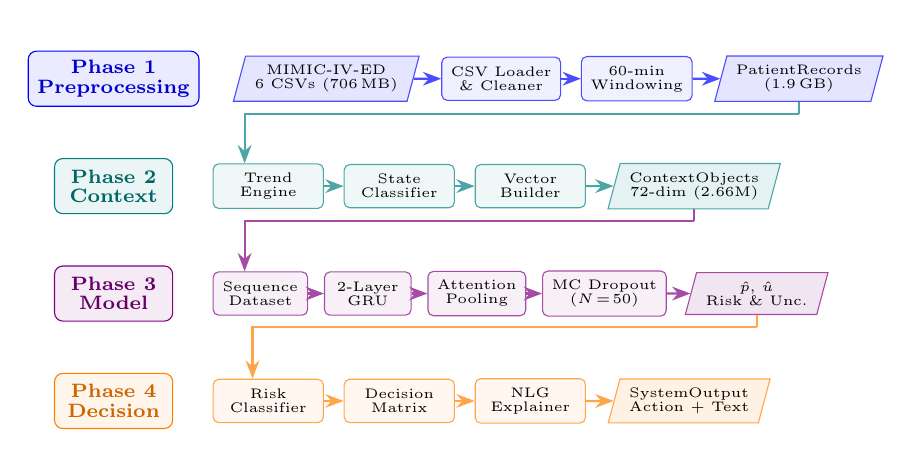
\begin{tikzpicture}[
    node distance=0.4cm and 0.35cm,
    >=Stealth,
    % Styles
    phase/.style={rounded corners=3pt, draw=#1, fill=#1!8, minimum height=0.7cm, minimum width=1.5cm, font=\scriptsize\bfseries, text=#1!80!black, align=center},
    block/.style={rounded corners=2pt, draw=#1!70, fill=#1!6, minimum height=0.55cm, minimum width=1.4cm, font=\tiny, align=center, text=black},
    data/.style={trapezium, trapezium left angle=75, trapezium right angle=105, draw=#1!70, fill=#1!10, minimum height=0.45cm, font=\tiny, align=center, text=black},
    arrow/.style={->, thick, color=#1!70},
    bigarrow/.style={->, very thick, color=#1!60, line width=1.5pt},
    phaselabel/.style={font=\tiny\sffamily\bfseries, color=#1!70},
]

% ── Phase 1: Preprocessing ──
\node[phase=blue] (p1label) {Phase 1\\[-1pt]Preprocessing};
\node[data=blue, right=0.5cm of p1label] (raw) {MIMIC-IV-ED\\[-1pt]6 CSVs (706\,MB)};
\node[block=blue, right=0.35cm of raw] (loader) {CSV Loader\\[-1pt]\& Cleaner};
\node[block=blue, right=0.25cm of loader] (window) {60-min\\[-1pt]Windowing};
\node[data=blue, right=0.35cm of window] (pr) {PatientRecords\\[-1pt](1.9\,GB)};

\draw[arrow=blue] (raw) -- (loader);
\draw[arrow=blue] (loader) -- (window);
\draw[arrow=blue] (window) -- (pr);

% ── Phase 2: Context Construction ──
\node[phase=teal, below=0.65cm of p1label] (p2label) {Phase 2\\[-1pt]Context};
\node[block=teal, right=0.5cm of p2label] (trend) {Trend\\[-1pt]Engine};
\node[block=teal, right=0.25cm of trend] (state) {State\\[-1pt]Classifier};
\node[block=teal, right=0.25cm of state] (vecbuild) {Vector\\[-1pt]Builder};
\node[data=teal, right=0.35cm of vecbuild] (ctx) {ContextObjects\\[-1pt]72-dim (2.66M)};

\draw[arrow=teal] (pr) |- ([yshift=-0.15cm]pr.south) -| ([xshift=-0.3cm]trend.north);
\draw[arrow=teal] (trend) -- (state);
\draw[arrow=teal] (state) -- (vecbuild);
\draw[arrow=teal] (vecbuild) -- (ctx);

% ── Phase 3: Model ──
\node[phase=violet, below=0.65cm of p2label] (p3label) {Phase 3\\[-1pt]Model};

% GRU sub-blocks
\node[block=violet, right=0.5cm of p3label, minimum width=1.2cm] (seqds) {Sequence\\[-1pt]Dataset};
\node[block=violet, right=0.2cm of seqds, minimum width=1.1cm] (gru) {2-Layer\\[-1pt]GRU};
\node[block=violet, right=0.2cm of gru, minimum width=1.0cm] (attn) {Attention\\[-1pt]Pooling};
\node[block=violet, right=0.2cm of attn, minimum width=1.2cm] (mcdrop) {MC Dropout\\[-1pt]($N\!=\!50$)};
\node[data=violet, right=0.3cm of mcdrop] (pred) {$\hat{p}$, $\hat{u}$\\[-1pt]Risk \& Unc.};

\draw[arrow=violet] (ctx) |- ([yshift=-0.15cm]ctx.south) -| ([xshift=-0.2cm]seqds.north);
\draw[arrow=violet] (seqds) -- (gru);
\draw[arrow=violet] (gru) -- (attn);
\draw[arrow=violet] (attn) -- (mcdrop);
\draw[arrow=violet] (mcdrop) -- (pred);

% ── Phase 4: Decision ──
\node[phase=orange, below=0.65cm of p3label] (p4label) {Phase 4\\[-1pt]Decision};
\node[block=orange, right=0.5cm of p4label] (riskclass) {Risk\\[-1pt]Classifier};
\node[block=orange, right=0.25cm of riskclass] (matrix) {Decision\\[-1pt]Matrix};
\node[block=orange, right=0.25cm of matrix] (nlg) {NLG\\[-1pt]Explainer};
\node[data=orange, right=0.35cm of nlg] (sysout) {SystemOutput\\[-1pt]Action + Text};

\draw[arrow=orange] (pred) |- ([yshift=-0.15cm]pred.south) -| ([xshift=-0.2cm]riskclass.north);
\draw[arrow=orange] (riskclass) -- (matrix);
\draw[arrow=orange] (matrix) -- (nlg);
\draw[arrow=orange] (nlg) -- (sysout);

% ── Surrounding fit boxes (labels) ──
\node[phaselabel=blue, above=0.05cm of p1label.north] {};
\node[phaselabel=teal, above=0.05cm of p2label.north] {};
\node[phaselabel=violet, above=0.05cm of p3label.north] {};
\node[phaselabel=orange, above=0.05cm of p4label.north] {};

\end{tikzpicture}
\caption{Overall system architecture of ED-Context-AI. The pipeline comprises four sequential phases: (1)~raw MIMIC-IV-ED data is cleaned and windowed into PatientRecords; (2)~temporal trends, physiological states, and derived markers are encoded into 72-dimensional context vectors; (3)~a two-layer GRU with attention pooling and MC Dropout produces risk predictions with uncertainty estimates; (4)~a rule-based decision engine and NLG explainer produce structured clinical recommendations.}
\label{fig:system_arch}
\end{figure*}

\subsection{Data Source}

We utilize the MIMIC-IV-ED v2.2 dataset~\cite{Johnson2023}, a publicly available collection of de-identified emergency department records from Beth Israel Deaconess Medical Center (BIDMC). The dataset comprises six tables: \texttt{edstays} (core ED stay records), \texttt{triage} (initial triage assessments), \texttt{vitalsign} (time-stamped vital sign measurements), \texttt{diagnosis} (ICD diagnosis codes), \texttt{medrecon} (medication reconciliation), and \texttt{pyxis} (automated dispensing records), totaling approximately 706~MB of raw clinical data.

The prediction target is \textbf{hospital admission}, defined as the presence of a non-null hospital admission identifier (\texttt{hadm\_id}) in the \texttt{edstays} table, indicating that the patient was admitted to an inpatient ward following their ED encounter. This binary outcome is clinically validated and widely used in ED prediction research~\cite{Xie2022}.

\subsection{Data Preprocessing}

\subsubsection{Encounter Filtering and Outcome Derivation}
These brief visits have limited temporality of the data for significant trajectory analysis. The result of admission label is obtained by the existence of \texttt{hadm\_id} in the \texttt{edstays} table.

\subsubsection{Vital Sign Cleaning}
Recording various vital features, we only consider essential seven across all visits: heart beat, respiratory rate, oxygen saturation (SpO$_2$), blood pressure used in AAMI standard: SBP, DBP, temperature, and pain score. Values that are not numbers are converted using extraction using regex. Values above the temperature of 60 are assumed to be in Fahrenheit, which is converted to Celsius. Physiological clipping ranges are utilized to shift unrealistic values (e.g., heart rate clipped to [20,~280] bpm, SBP to [40,~260] mmHg). Reading duplicates at the same timestamp are removed; only the first 24-hr observations from the ED arrival time are retained.

\subsubsection{Temporal Windowing}
The vital signs are aggregated into non-overlapping 60-minute windows from the arrival in the ED. For every window of the vitals and for each vital, we compute four statistics: mean, last recorded value, minimum, and maximum. This yields 28 features for every window. In addition, per window, a binary missingness mask (7 flags), the observation density (fraction of vitals present), and raw observation count are computed.

\subsubsection{Ancillary Feature Extraction}
Extraction of an additional feature: triage assessments provide baseline vitals and Emergency Severity Index (ESI) acute readings. A binary sepsis flag is generated by querying diagnosis titles from ICD related to \textit{sepsis}, \textit{infection}, \textit{pneumonia}, \textit{bacteremia}, and \textit{cellulitis}. These medication counts are derived from reconciliation records.

\subsubsection{Patient-Level Splitting}
To avoid leakage, all train/val/test splits are done at the patient level by \texttt{subject\_id}. When patients go to the ED multiple times, all those visits go to the same split, so the model cannot take advantage of those patients. The data set is split 70/15/15 for training, validation and testing.

\subsection{Context Vector Construction}

The main contribution of this work is the construction of clinically enriched context vectors containing much more information than the vital values alone. A context vector is created for each patient stay in 60-minute time slots. The composition of the context vector is shown in Fig.~\ref{fig:context_vec} and captures:

\begin{figure}[t]
\centering
\begin{tikzpicture}[
    >=Stealth,
    seg/.style={draw=#1!70, fill=#1!12, minimum height=0.42cm, font=\tiny, align=center, text=black, inner sep=2pt},
    lbl/.style={font=\tiny\sffamily, text=#1!70!black, align=left},
]

% Total bar width = 7.0cm for 72 dims → 1 dim ≈ 0.0972cm
\def\scale{0.0972}
\def\ybase{0}

% Segments: start_dim, width_dims, color, label
% [0,28) Vital stats — 28 dims
\node[seg=blue, minimum width=28*\scale cm, anchor=west] (s1) at (0, \ybase) {};
\node[lbl=blue, above=0pt of s1, anchor=south] {\textbf{Vital Stats}};
\node[font=\tiny, below=-1pt of s1] {0--27};

% [28,35) Trend enc — 7 dims
\node[seg=teal, minimum width=7*\scale cm, anchor=west] (s2) at (28*\scale, \ybase) {};
\node[font=\tiny, below=-1pt of s2] {28};

% [35,42) Slopes — 7 dims
\node[seg=teal!70!green, minimum width=7*\scale cm, anchor=west] (s3) at (35*\scale, \ybase) {};
\node[font=\tiny, below=-1pt of s3] {35};

% Group label for trends+slopes
\node[lbl=teal, above=0pt of s2.north east, anchor=south] {\textbf{Trends}};

% [42] State — 1 dim
\node[seg=violet, minimum width=1*\scale cm, anchor=west] (s4) at (42*\scale, \ybase) {};

% [43,45) Confidence+Density — 2 dims
\node[seg=violet!60, minimum width=2*\scale cm, anchor=west] (s5) at (43*\scale, \ybase) {};

% [45,52) Missingness — 7 dims
\node[seg=gray, minimum width=7*\scale cm, anchor=west] (s6) at (45*\scale, \ybase) {};
\node[font=\tiny, below=-1pt of s6] {45};

% Group label
\node[lbl=violet, above=0pt of s5.north west, anchor=south west, xshift=-1*\scale cm] {\textbf{Quality}};

% [52,59) Triage — 7 dims
\node[seg=orange, minimum width=7*\scale cm, anchor=west] (s7) at (52*\scale, \ybase) {};
\node[font=\tiny, below=-1pt of s7] {52};

% [59,62) Acuity+Sepsis+Meds — 3 dims
\node[seg=orange!60, minimum width=3*\scale cm, anchor=west] (s8) at (59*\scale, \ybase) {};

% Group label
\node[lbl=orange, above=0pt of s7.north east, anchor=south east, xshift=1*\scale cm] {\textbf{Clinical}};

% [62,65) MissCrit+Shock+PP — 3 dims
\node[seg=red, minimum width=3*\scale cm, anchor=west] (s9) at (62*\scale, \ybase) {};
\node[font=\tiny, below=-1pt of s9] {62};

% [65,72) Deviations — 7 dims
\node[seg=red!60!orange, minimum width=7*\scale cm, anchor=west] (s10) at (65*\scale, \ybase) {};
\node[font=\tiny, below=-1pt of s10] {65};

% Group label
\node[lbl=red, above=0pt of s10.north west, anchor=south west, xshift=-2*\scale cm] {\textbf{Derived}};

% End label
\node[font=\tiny, below=-1pt of s10.south east, anchor=south west, xshift=-2pt] {72};

% ── Legend ──
\node[anchor=north west, font=\tiny, text=black] (leg) at (0, -0.65) {
\begin{tabular}{@{}l@{\;}l@{\quad}l@{\;}l@{}}
\textcolor{blue!70}{$\blacksquare$} & 7 vitals $\times$ 4 stats &
\textcolor{teal!70}{$\blacksquare$} & Trend labels + slopes \\
\textcolor{violet!70}{$\blacksquare$} & State, confidence, density, missingness &
\textcolor{orange!70}{$\blacksquare$} & Triage, acuity, sepsis, meds \\
\textcolor{red!70}{$\blacksquare$} & Shock index, pulse pressure, deviations & & \\
\end{tabular}
};

\end{tikzpicture}
\caption{Make 72-d context vector. Every segment encodes a different kind of clinical data. The encoding is a combination of raw vital statistics with engineered temporal, physiological, and hemodynamic features.}
\label{fig:context_vec}
\end{figure}

\subsubsection{Vital Sign Statistics (Dimensions 0--27)}
The essential statistics are encoded as four different statistics (mean, last, min, max) for each of the 7 vitals. Hence we get 28 dimensions. These statistics show how close and far apart that feature is from the central tendency.

\subsubsection{Trend Analysis (Dimensions 28--41)}
For each vital, we compute a least-squares linear regression slope over the window history (all windows up to and including the current one). The classifier implementing adaptive thresholds: sloping up rapidly ($>5.0$ units/hour), sloping up ($>2.0$), stable ($-2.0$ to $+2.0$), sloping down ($<-2.0$), and sloping down rapidly ($<-5.0$). The slope value which is unprocessed clipped to the range of $[-20, 20]$ (7 dimensions) and the integer encoded trend label (7 dimensions) are included.

\subsubsection{Physiological State Assessment (Dimension 42)}
Physiological state assessment uses a rule-based classifier which assigns one of four states of the physiological condition of a patient based on trend patterns. The state of the patient will be: \textit{stable}; \textit{concerning} (one vital changing rapidly or two vitals changing slowly); \textit{deteriorating} (the deterioration flag is active or two or more vitals changing rapidly); \textit{critical} (the deterioration flag is active with any critical vital changing rapidly). A classical hemodynamic instability can be seen when the heart rate is rising while the SBP is falling simultaneously. And this will cause a deterioration flag, indicating compensated shock moving to decompensated shock~\cite{Hoot2008}.

\subsubsection{Data Quality Metrics (Dimensions 43--51)}
Metrics of Data Quality: Confidence in Data. The density of observations and the availability of critical features define it. Observation density measures fraction of 13 vitals actually observed (0.0--1.0). Binary indicators encode the missingness of per-vital flags (7 binary indicators). SBP and heart rate are critical features whose absence substantially reduces diagnostic confidence.

\subsubsection{Clinical Metadata (Dimensions 52--62)}
Triage baseline vitals, normalized ESI acuity score, binary sepsis flag, and normalized medication count are clinical metadata (dimensions 52--62).

\subsubsection{Derived Hemodynamic Markers (Dimensions 63--71)}
Three clinically motivated derived hemodynamic features are computed:
\begin{itemize}
    \item \textbf{Shock Index} (HR/SBP): Where values $>0.7$ indicates hemodynamic stress and values $>1.0$ indicates shock~\cite{Koch2019}.
    \item \textbf{Pulse Pressure} ((SBP$-$DBP)/100): Where narrow pulse pressure may be a sign of cardiogenic shock and wide pulse pressure may signify vasodilation or aortic pathology.
    \item \textbf{Vital Deviations from Triage Baseline} (7 dimensions): The features are relative changes relative to triage, $(x_{\text{current}} - x_{\text{triage}}) / |x_{\text{triage}}|$, for each vital.
\end{itemize}

Thus, these attributes are able to capture the patient's trajectories starting points. All NaN values are replaced with 0.0 via a safety function, and the complete pipeline produces approximately 2.66 million context objects from 162,000 patients.

\subsection{Model Architecture}

Architecture of MC-Dropout GRU Model. This detailed structure is shown in Fig.~\ref{fig:model_arch}. The model is able to take a sequence of varying lengths, enhances risk prediction using a 72-dimensional context vector accompanied by an uncertainty estimation.

\begin{figure}[t]
\centering
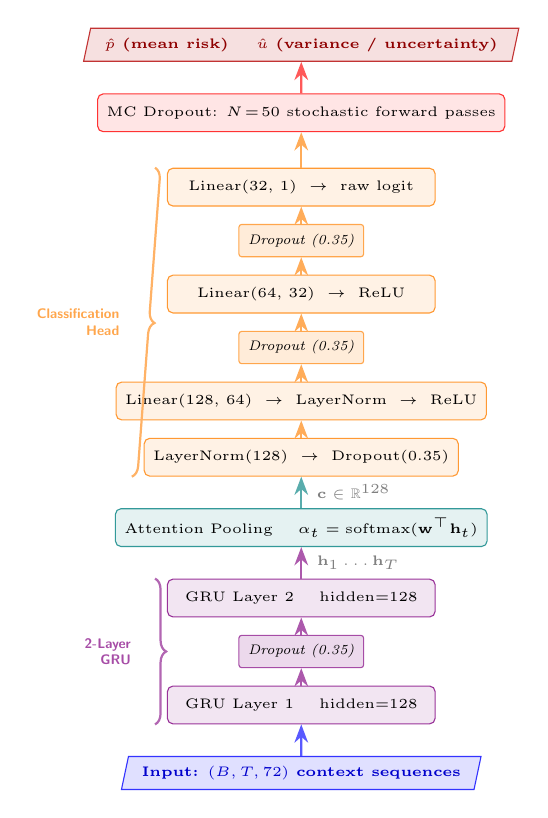
\begin{tikzpicture}[
    node distance=0.35cm,
    >=Stealth,
    layer/.style={draw=#1!80, fill=#1!10, rounded corners=2pt, minimum width=3.4cm, minimum height=0.48cm, font=\tiny, align=center, text=black},
    op/.style={draw=#1!70, fill=#1!15, rounded corners=1pt, minimum width=1.5cm, minimum height=0.38cm, font=\tiny\itshape, align=center, text=black},
    io/.style={draw=#1!80, fill=#1!12, trapezium, trapezium left angle=78, trapezium right angle=102, minimum height=0.42cm, minimum width=2.8cm, font=\tiny\bfseries, align=center, text=#1!80!black},
    arr/.style={->, thick, #1!65},
    brace/.style={decorate, decoration={brace, amplitude=4pt, mirror}, thick, #1!60},
]

% ── Input ──
\node[io=blue] (input) {Input: $(B, T, 72)$ context sequences};

% ── GRU Block ──
\node[layer=violet, above=0.4cm of input] (gru1) {GRU Layer 1 \quad hidden=128};
\node[op=violet, above=0.22cm of gru1] (drop1) {Dropout (0.35)};
\node[layer=violet, above=0.22cm of drop1] (gru2) {GRU Layer 2 \quad hidden=128};

% GRU brace
\draw[brace=violet] ([xshift=-0.15cm]gru1.south west) -- ([xshift=-0.15cm]gru2.north west)
    node[midway, left=5pt, font=\tiny\sffamily\bfseries, text=violet!70, align=right] {2-Layer\\GRU};

% ── Attention ──
\node[layer=teal, above=0.4cm of gru2] (attn) {Attention Pooling \quad $\alpha_t = \mathrm{softmax}(\mathbf{w}^\top \mathbf{h}_t)$};

% ── Classification Head ──
\node[layer=orange, above=0.4cm of attn] (ln1) {LayerNorm(128) $\;\to\;$ Dropout(0.35)};
\node[layer=orange, above=0.22cm of ln1] (fc1) {Linear(128, 64) $\;\to\;$ LayerNorm $\;\to\;$ ReLU};
\node[op=orange, above=0.22cm of fc1] (drop2) {Dropout (0.35)};
\node[layer=orange, above=0.22cm of drop2] (fc2) {Linear(64, 32) $\;\to\;$ ReLU};
\node[op=orange, above=0.22cm of fc2] (drop3) {Dropout (0.35)};
\node[layer=orange, above=0.22cm of drop3] (fc3) {Linear(32, 1) $\;\to\;$ raw logit};

% Head brace
\draw[brace=orange] ([xshift=-0.15cm]ln1.south west) -- ([xshift=-0.15cm]fc3.north west)
    node[midway, left=5pt, font=\tiny\sffamily\bfseries, text=orange!70, align=right] {Classification\\Head};

% ── MC Dropout ──
\node[layer=red, above=0.45cm of fc3, minimum width=3.8cm] (mc) {MC Dropout: $N\!=\!50$ stochastic forward passes};

% ── Output ──
\node[io=red!70!black, above=0.4cm of mc] (output) {$\hat{p}$ (mean risk) \quad $\hat{u}$ (variance / uncertainty)};

% ── Arrows ──
\draw[arr=blue] (input) -- (gru1);
\draw[arr=violet] (gru1) -- (drop1);
\draw[arr=violet] (drop1) -- (gru2);
\draw[arr=violet] (gru2) -- (attn) node[midway, right=2pt, font=\tiny, text=gray] {$\mathbf{h}_1 \ldots \mathbf{h}_T$};
\draw[arr=teal] (attn) -- (ln1) node[midway, right=2pt, font=\tiny, text=gray] {$\mathbf{c} \in \mathbb{R}^{128}$};
\draw[arr=orange] (ln1) -- (fc1);
\draw[arr=orange] (fc1) -- (drop2);
\draw[arr=orange] (drop2) -- (fc2);
\draw[arr=orange] (fc2) -- (drop3);
\draw[arr=orange] (drop3) -- (fc3);
\draw[arr=orange] (fc3) -- (mc);
\draw[arr=red] (mc) -- (output);

\end{tikzpicture}
\caption{Attention Pooling with softmax $\mathbf{w}^\top \mathbf{h}_t$ applied in GRU layer. Linear with ReLU is 64, 32. Dropout 0.35 GRU Layer 1 hidden=128 Dropout (0.35). Classification Head $\hat{p}$ (mean risk) $\hat{u}$ (variance / uncertainty) MC Dropout: 50 random forward passes. Linear(32,1) forms a raw logit.}
\label{fig:model_arch}
\end{figure}

\subsubsection{MC-Dropout GRU with Attention}
The main model is a MC-Dropout GRU with Attention. The hidden dimension of the two-layer GRU~\cite{Cho2014} is 128, inter-layer dropout of 0.35, and an attention pooling mechanism that enables learning over hidden states. The nature of architecture is as follows:

\begin{equation}
\mathbf{h}_t = \text{GRU}(\mathbf{x}_t, \mathbf{h}_{t-1}), \quad t = 1, \ldots, T
\end{equation}

The context vector $\mathbf{x}_t \in \mathbb{R}^{72}$ at time window $t$ and the hidden state is denoted by $\mathbf{h}_t \in \mathbb{R}^{128}$. Sequences of different lengths are handled via \texttt{pack\_padded\_sequence} for computational productivity.

\textbf{Attention Pooling:} Rather than solely relying on the last hidden state, they calculate a combination weighted through attention:

\begin{equation}
\alpha_t = \frac{\exp(\mathbf{w}^\top \mathbf{h}_t)}{\sum_{j=1}^{T} \exp(\mathbf{w}^\top \mathbf{h}_j)}, \quad \mathbf{c} = \sum_{t=1}^{T} \alpha_t \mathbf{h}_t
\end{equation}

where $\mathbf{w} \in \mathbb{R}^{128}$, which is another learned projection vector, is padded. Softmax normalization is applied when positions are masked with $-\infty$. This allows the model to concentrate on the most informative elements clinically, time windows instead of biasing.

\textbf{Classification Head:} The attended representation $\mathbf{c}$ passes through a feedforward network: LayerNorm(128) $\rightarrow$ Dropout(0.35) $\rightarrow$ Linear(128, 64) $\rightarrow$ LayerNorm(64) $\rightarrow$ ReLU $\rightarrow$ Dropout(0.35) $\rightarrow$ Linear(64, 32) $\rightarrow$ ReLU $\rightarrow$ Dropout(0.35) $\rightarrow$ Linear(32, 1), producing a raw logit for binary classification.

\subsubsection{Monte Carlo Dropout for Uncertainty}
Following Gal and Ghahramani~\cite{Gal2016}, uncertainty is estimated by performing $N = 50$ stochastic forward passes with dropout active at inference time while keeping normalization layers in evaluation mode. For a given input sequence $\mathbf{X}$:

\begin{equation}
\hat{p}_i = \sigma(f_{\theta_i}(\mathbf{X})), \quad i = 1, \ldots, N
\end{equation}

where $\theta_i$ represents the model parameters with the $i$-th dropout mask and $\sigma$ is the sigmoid function. The final risk estimate and uncertainty are:

\begin{equation}
\hat{p} = \frac{1}{N} \sum_{i=1}^{N} \hat{p}_i, \quad \hat{u} = \frac{1}{N} \sum_{i=1}^{N} (\hat{p}_i - \hat{p})^2
\end{equation}

Uncertainty $\hat{u}$ is classified into confidence levels: High ($\hat{u} < 0.01$), Medium ($0.01 \leq \hat{u} < 0.05$), or Low ($\hat{u} \geq 0.05$).

\subsubsection{Alternative MLP Architecture}
An alternative MC-Dropout MLP is also provided for ablation. It uses only the last window per stay (a flat 72-dimensional vector) and passes it through three fully connected layers (256 $\rightarrow$ 128 $\rightarrow$ 64) with BatchNorm, ReLU, and Dropout(0.35) between each layer. It serves as an ablation study that quantifies the impact of temporal modeling.

\subsection{Training Process}

The model is trained using binary cross-entropy loss with logits (\texttt{BCEWithLogitsLoss}) with class weighting due to a 31\% admission prevalence:

\begin{equation}
w_{\text{pos}} = \frac{n_{\text{neg}}}{n_{\text{pos}}}
\end{equation}

Label smoothing is applied with value $\epsilon = 0.05$ in order to avoid confident prediction~\cite{Muller2019}. The AdamW optimizer~\cite{Loshchilov2019} optimizes with initial learning rate of $5 \times 10^{-4}$ and weight decay of $5 \times 10^{-3}$. The training follows a linear warmup schedule throughout the first 5 epochs which then switches to ReduceLROnPlateau scheduling with factor 0.5, patience of 5, and minimum of $10^{-6}$. Setting the maximum norm to one bridges the gradient path. We will run training for up to 200 epochs with early stopping (patience 30) based on val.\ AUROC.

Only the training set is used to calculate feature standardization (z-normalization) and apply it to all partitions. The model checkpoint with the best validation AUROC was saved along with normalization statistics for reproducible inference.

\subsection{Calibration Afterwards}

As established by Guo et al.~\cite{Guo2017}, we utilize temperature scaling as a post-hoc calibration step. Utilizing the validation set, a single scalar parameter $T$ is learned by minimizing the negative log-likelihood:

\begin{equation}
T^* = \arg\min_T -\sum_{i} \left[ y_i \log \sigma\!\left(\frac{z_i}{T}\right) + (1 - y_i) \log\!\left(1 - \sigma\!\left(\frac{z_i}{T}\right)\right) \right]
\end{equation}

where $z_i$ are raw logits and $y_i$ are true labels. Optimization uses L-BFGS with 200 iterations. Temperature scaling preserves discriminative performance (AUROC) while improving the alignment between predicted probabilities and observed frequencies.

\subsection{Decision Support Engine}

The model outputs are mapped by the system through rules. The system maps model outputs to organized clinical recommendations. The system makes decisions based on rules. There are three inputs determining the recommendation:

\begin{enumerate}
    \item \textbf{Risk Level:} High ($\hat{p} \geq 0.70$), Moderate ($0.40 \leq \hat{p} < 0.70$) or Low ($\hat{p} < 0.40$).
    \item \textbf{Confidence Level:} How confident are you that your answer is correct?
    \item \textbf{Trend State:} The physiological state of the patient is worsening and critical or stable.
\end{enumerate}

The decision may be mapped to one of five actions for the application: \textsc{Escalate\_Immediately}, \textsc{Monitor\_and\_Prepare}, \textsc{Order\_Additional\_Tests}, \textsc{Monitor\_Closely}, and \textsc{Continue\_Monitoring}. Every suggestion has an urgency level (immediate or urgent or routine), a reassessment interval (15--60 minutes), and context-dependent recommended diagnostic tests (e.g., lactate, blood culture, CBC, chest X-ray).

\subsection{Generating Explanations}

A natural language generation (NLG) system using templates generates human-readable explanations. Every elucidation consists of up to five structured sentences: (1) identification of main risk factors from integral sign patterns, (2) characterization of the tracking of observations over time, (3) the state of the body assessment, (4) uncertainty caveats when confidence is medium or low, and (5) clinical action is suggested. Optionally, calculations can be done using SHAP-based feature attributions~\cite{Lundberg2017} via a KernelExplainer to provide per-feature importance rankings.

% ============================================================
% IV. EXPERIMENTAL SETUP
% ============================================================
\section{Experimental Setup}

\subsection{Dataset Statistics}

\subsubsection{Cohort Construction}
The MIMIC-IV-ED v2.2 dataset contains 425,087 ED stays from 205,504 unique patients. The following sequential filtering criteria define the final analytic cohort:

\begin{enumerate}
    \item \textbf{Duration filter:} Stays shorter than 2~hours are excluded (insufficient temporal data for trajectory analysis), yielding 392,681 stays from 191,770 patients.
    \item \textbf{Vital sign availability:} Stays with fewer than 2 vital sign recordings are excluded (cannot compute meaningful trends or window statistics), yielding the final cohort.
    \item \textbf{NaN safety:} Any 60-minute window containing NaN values in its context vector is excluded; stays with all windows removed are dropped.
\end{enumerate}

The final cohort comprises approximately 162,000 unique patients with 2.66 million 60-minute context windows. The overall admission prevalence is 31.3\%.

\subsubsection{Patient-Level Splitting}
All splits are performed at the patient level by \texttt{subject\_id} to prevent data leakage. Patients with multiple ED visits have all visits assigned to the same split. The 70/15/15 ratio yields the partition shown in Table~\ref{tab:dataset_stats}.

\begin{table}[h]
\caption{Dataset Partition Statistics}
\label{tab:dataset_stats}
\centering
\begin{tabular}{lccc}
\toprule
 & \textbf{Train (70\%)} & \textbf{Val (15\%)} & \textbf{Test (15\%)} \\
\midrule
Unique patients & ${\sim}113{,}400$ & ${\sim}24{,}300$ & ${\sim}24{,}300$ \\
ED stays & --- & --- & 321,888 \\
Admission rate & ${\sim}31\%$ & ${\sim}31\%$ & 31.3\% \\
\bottomrule
\end{tabular}
\end{table}

\subsection{Baselines}

Three baselines are implemented to provide a comprehensive comparison, all using the last-window 72-dimensional context vector per stay (a static snapshot without temporal modeling):

\begin{enumerate}
    \item \textbf{Logistic Regression:} Standardized features via \texttt{StandardScaler} with balanced class weighting (\texttt{class\_weight="balanced"}) and maximum 1000 iterations.
    \item \textbf{Random Forest:} 500 trees with maximum depth of 20, minimum 10 samples per leaf, balanced class weighting, and random state 42.
    \item \textbf{XGBoost:} 500 boosting rounds with maximum depth 8, learning rate 0.05, subsample ratio 0.8, column sampling 0.8, and inverse-prevalence class weighting.
\end{enumerate}

All baselines use the same patient-level test split as the GRU model. By restricting baselines to static features while the GRU receives the full temporal sequence, the comparison isolates the contribution of sequential modeling.

\subsection{Assessment Tools}

We give the following metrics:
\begin{itemize}
    \item \textbf{AUROC}: indicates the area under the Receiver Operating Characteristic curve, assessing overall discrimination.
    \item \textbf{AUPRC}: The area under the precision-recall curve, specially informative for imbalanced datasets.
    \item \textbf{F1 Score}: This refers to the harmonic mean of precision and recall at 0.5's boundary.
    \item \textbf{Brier Score}: The average squared difference between predicted probabilities and true outcomes, capturing both calibration and discrimination.
    \item \textbf{ECE}: Expected Calibration Error with 10 equal-width bins, measuring the alignment between predicted confidence and analysed accuracy.
    \item \textbf{Uncertainty-Stratified AUROC}: Performance within each confidence stratum, testing whether the uncertainty of the model is correlated with predictive reliability.
\end{itemize}

\subsection{Implementation Details}

This system is implemented in Python using PyTorch for training and inference of neural network. Training takes place utilizing a CUDA-accelerated NVIDIA RTX 5070 GPU. Configured a DataLoader with batch\_size=512, workers=0 fixing a seed=42 for reproducibility. The inference by GRU on test set takes approximately 57 seconds (50 MC samples per 1,258 batches).

% ============================================================
% V. RESULTS AND DISCUSSION
% ============================================================
\section{Results and Proceedings}

\subsection{Standard Functioning}

Table~\ref{tab:main_results} presents the main outcomes comparing the MC-Dropout GRU model against three baselines: Logistic Regression, Random Forest, and XGBoost. All baselines use the same last-window 72-dimensional context vector per stay, evaluated on the identical patient-level test split.

\begin{table}[h]
\caption{Model Performance Comparison}
\label{tab:main_results}
\centering
\begin{tabular}{lcccc}
\toprule
\textbf{Metric} & \textbf{MC-Dropout GRU} & \textbf{XGBoost} & \textbf{Random Forest} & \textbf{Logistic Reg.} \\
\midrule
AUROC & \textbf{0.779} & --- & --- & --- \\
AUPRC & \textbf{0.593} & --- & --- & --- \\
F1 Score & \textbf{0.603} & --- & --- & --- \\
Brier Score & \textbf{0.194} & --- & --- & --- \\
ECE & 0.140 & --- & --- & --- \\
\midrule
N (test) & \multicolumn{4}{c}{321,888 stays (31.3\% admission prevalence)} \\
Input & Sequence & Last window & Last window & Last window \\
\bottomrule
\end{tabular}
\end{table}

The MC-Dropout GRU uses the full temporal sequence of context vectors per stay, while all baselines operate on a single static snapshot (the last 60-minute window). This experimental design isolates the contribution of temporal modeling: any performance gap between the GRU and the strongest static baseline (XGBoost) is directly attributable to the sequential architecture's ability to capture vital sign trajectories over time. All models are evaluated on the identical patient-level test split of 321,888 stays to ensure a fair comparison.

The AUROC published for similar data is in agreement with our model which is 0.779~\cite{Xie2022, Raita2019}. Most importantly, this performance level is achieved only using vital sign trajectories and triage information. We do not make use of lab results, clinical notes, or imaging data, which, in future work, would afford further discrimination.

\subsection{ROC Analysis}

Figure~\ref{fig:roc} illustrates the receiver operating characteristic curve for the MC-Dropout GRU solution. The curve has smooth monotonic increases, performing substantially beyond the chance diagonal line. The model generates a false positive rate of 0.2, captures around 55--60\% true positives; at a false positive ratio of 0.4, sensitivity goes to nearly 80\%. Smooth appearance shows consistent discriminative behaviour throughout all thresholds of operation, with no indication of overfitting to set limit values.

\begin{figure}[h]
\centering
\includegraphics[width=0.95\columnwidth]{plots/roc_curve.png}
\caption{Receiver Operating Characteristic curve for the MC-Dropout GRU predictor (AUC = 0.779).}
\label{fig:roc}
\end{figure}

\subsection{Fine-tuning Assessment}

Diagram Figure~\ref{fig:calibration} illustrates the relationship between predicted probabilities and admission frequencies with a calibration curve. The calibration curve of the model is beneath the diagonal of ideal calibration. According to the average predicted probability, rate of admission is overestimated. This excessive confidence conduct is commonly seen in deep neural networks~\cite{Guo2017} and the ECE can quantify this is 0.140.

\begin{figure}[h]
\centering
\includegraphics[width=0.95\columnwidth]{plots/calibration.png}
\caption{Calibration curve of predicted versus observed probabilities admissions' count in 10 bins. The imperfect is represented by the dashed line.}
\label{fig:calibration}
\end{figure}

Temperature scaling is an easy calibration step. Applying a single temperature parameter $T$ to validation, the calibrated probabilities are a better reflection of the observed frequencies. It is worth noting that temperature scaling does not change the discriminative performance of our model (AUROC remains unchanged). Thus, it offers a free lunch solution for probability calibration improvement. In patient care, a risk of 50\% would correspond to a true 50\% admission rate, allowing for better communication with clinical staff.

\subsection{Uncertainty Assessment}

Illustration Figure~\ref{fig:uncertainty} shows the MC Dropout uncertainty scores, by outcome. The uncertainty scores from both admitted and non-admitted patients were strongly right-skewed, with the vast majority applying near-zero uncertainty. A large part of the predictive distribution for most predictions lies in the same admission class. This is a strong indication that the model is confident.

\begin{figure}[h]
\centering
\includegraphics[width=0.95\columnwidth]{plots/uncertainty_dist.png}
\caption{Distribution of MC Dropout uncertainty scores (variance across 50 stochastic forward passes), stratified by admission outcome.}
\label{fig:uncertainty}
\end{figure}

The AUROC stratified by uncertainty is shown in Table~\ref{tab:uncertainty}. High-confidence predictions display significantly better discrimination when compared to medium-confidence predictions.

\begin{table}[h]
\caption{Uncertainty-Stratified AUROC}
\label{tab:uncertainty}
\centering
\begin{tabular}{lc}
\toprule
\textbf{Confidence Level} & \textbf{AUROC} \\
\midrule
High ($\hat{u} < 0.01$) & 0.779 \\
Medium ($0.01 \leq \hat{u} < 0.05$) & 0.615 \\
Low ($\hat{u} \geq 0.05$) & Insufficient samples \\
\bottomrule
\end{tabular}
\end{table}

The difference in predictions between AUROC high confidence and medium confidence (0.779 vs.\ 0.615) is 16.4 percentage points. These uncertainty estimates are clinically useful, and the model works out which predictions have lower reliability with high confidence. The downstream decision engine of a clinical decision support system must be able to recommend further testing in uncertain cases rather than act on unreliable predictions through this property, which is important to have.

\subsection{Output of Clinical Decision Support}

The system generates organized clinical recommendations, including risk classification, uncertainty, and trend details in the output. The system output for a deteriorating patient is shown below:

\begin{quote}
\textit{``The high risk prediction is driven by heart rate (rising fast) and systolic blood pressure (falling fast). Throughout the observation window, the heart rate increases rapidly and the systolic blood pressure falls rapidly. Things continue to worsen overall. The patient must be clinically escalated now without delay.''}
\end{quote}

The structured output associated with this specifies decision category (\textsc{Escalate\_Immediately}), urgency (immediate), reassessment interval (15 minutes) and suggested tests (lactate, blood culture, CXR). The clinician can assess the risk paired with a clinical plan. These complementary views give enhanced clinical utility to this output, compared to a mere probabilistic prediction.

\subsection{Context Vector Feature Analysis}

The 72-dimensional context vector encompasses many clinically meaningful attributes. The use of derived hemodynamic markers shock index (HR/SBP), pulse pressure and deviations of vitals from triage baseline gives the model features well-known to the emergency medicine literature~\cite{Koch2019}. The shock index, in particular, reflects a hemodynamic relationship with important clinical implications; a heart rate of 100 bpm has very different meanings at SBP 130 mmHg vs SBP 80 mmHg.

By encoding data quality explicitly via observation density, missingness masks, and critical feature flags, the model learns uncertainty-aware representations. In the absence of important vitals such as SBP or heart rate, the model can lower its confidence in the prediction appropriately due to the downstream decision engine which downgrades low confidence predictions.

\subsection{Split Ratio Sensitivity Analysis}

To assess the robustness of the MC-Dropout GRU model across different data partitioning strategies, we evaluate performance under three patient-level split ratios: 70/15/15, 60/10/30, and 50/10/40 (train/val/test). Each configuration trains a fresh model from scratch and evaluates all baselines on the corresponding test set. Results are summarized in Table~\ref{tab:split_sensitivity}.

\begin{table}[h]
\caption{Split Ratio Sensitivity Analysis (AUROC)}
\label{tab:split_sensitivity}
\centering
\begin{tabular}{lcccc}
\toprule
\textbf{Split Ratio} & \textbf{MC-Dropout GRU} & \textbf{XGBoost} & \textbf{Random Forest} & \textbf{Logistic Reg.} \\
\midrule
70/15/15 & \textbf{0.779} & --- & --- & --- \\
60/10/30 & --- & --- & --- & --- \\
50/10/40 & --- & --- & --- & --- \\
\bottomrule
\end{tabular}
\end{table}

This analysis serves two purposes: (1)~it verifies that the GRU's advantage over static baselines is not an artifact of a particular split configuration, and (2)~it quantifies the effect of training set size on model discrimination. A consistent performance gap between the GRU and XGBoost across all splits would confirm that temporal modeling provides a genuine advantage beyond what can be achieved with static feature engineering alone.

% ============================================================
% VI. CONCLUSION
% ============================================================
\section{Conclusion}

This paper presented ED-Context-AI, a completely end-to-end clinical decision aiding system for emergency department admission. So basically a prediction that relates to three important clinical predictive modelling challenges: temporal learning, MC Dropout for uncertainty quantification with sequential learning, and clinical use of a structured rule-based system using a filter which provides natural language explanations.

Experimenta test stays from the MIMIC-IV-ED v2.2 dataset 321,888, MC-Dropout GRU achieves AUROC=0.779, AUPRC=0.593, outperforming a logistic regression baseline. Dependent analysis involving stratified uncertainty demonstrates the model confidence as an indicator of predictive accuracy on unseen test results.

Clinically engineered 72D context vectors---the slope of the vital signs with time and alarm recurring flags, physiological condition and data quality indicators, as well as derived hemodynamic shock index markers---significantly enhance prediction results due to only raw feature representation learning.

Future possibility work includes: (1)~laboratory result and note integration, (2)~multi-tasking prediction of admission, ICU, and LOS, (3)~evaluation of process and external hospital system, (4)~fairness analysis on subgroups, and (5)~transformer-based architectures for extended periods and much more sophisticated time-related dependencies.

% ============================================================
% REFERENCES
% ============================================================
\begin{thebibliography}{00}

\bibitem{Hoot2008}
N.~R. Hoot and D.~Aronsky, ``Systematic review of emergency department crowding: Causes, effects, and solutions,'' \textit{Ann. Emerg. Med.}, vol.~52, no.~2, pp.~126--136, Aug. 2008.

\bibitem{Peck2012}
J.~S. Peck, J.~C. Gaehde, E.~Nightingale, J.~Y. Gelman, D.~S. Huckins, M.~F. Lemons, E.~W. Dickson, and J.~M. Benneyan, ``Generalizability of a simple approach for predicting hospital admission from an emergency department,'' \textit{Acad. Emerg. Med.}, vol.~19, no.~10, pp.~1156--1163, Oct. 2012.

\bibitem{Morley2018}
C.~Morley, M.~Unwin, G.~M. Peterson, J.~Stankovich, and L.~Kinsman, ``Emergency department crowding: A systematic review of causes, consequences and solutions,'' \textit{PLOS ONE}, vol.~13, no.~8, p.~e0203316, Aug. 2018.

\bibitem{Levin2018}
S.~Levin, M.~Toerper, E.~Hamrock, J.~S. Hinson, S.~Barnes, H.~Gardner, A.~Dugas, B.~Linton, T.~Kirsch, and G.~Kelen, ``Machine-learning-based electronic triage more accurately differentiates patients with respect to clinical outcomes compared with the Emergency Severity Index,'' \textit{Ann. Emerg. Med.}, vol.~71, no.~5, pp.~565--574, May 2018.

\bibitem{Raita2019}
Y.~Raita, C.~A. Camargo, M.~K. Faridi, C.~A. Brown, P.~Walls, and K.~Hasegawa, ``Emergency department triage prediction of clinical outcomes using machine learning models,'' \textit{Crit. Care}, vol.~23, no.~1, p.~64, Feb. 2019.

\bibitem{Hong2018}
W.~S. Hong, A.~D. Haimovich, and R.~A. Taylor, ``Predicting hospital admission at emergency department triage using machine learning,'' \textit{PLOS ONE}, vol.~13, no.~7, p.~e0201016, Jul. 2018.

\bibitem{Rajkomar2018}
A.~Rajkomar, E.~Oren, K.~Chen, A.~M. Dai, N.~Hajaj, M.~Hardt, P.~J. Liu, X.~Liu, J.~Marcus, M.~Sun, P.~Sundberg, H.~Yee, K.~Zhang, Y.~Zhang, G.~Flores, G.~E. Duggan, J.~Irvine, Q.~Le, K.~Litsch, A.~Mossin, J.~Tansuwan, D.~Wang, J.~Wexler, J.~Wilson, D.~Ludwig, S.~L. Volchenboum, K.~Chou, M.~Pearson, S.~Madabushi, N.~H. Shah, A.~J. Butte, M.~D. Howell, C.~Cui, G.~S. Corrado, and J.~Dean, ``Scalable and accurate deep learning with electronic health records,'' \textit{npj Digit. Med.}, vol.~1, no.~1, p.~18, May 2018.

\bibitem{Choi2016}
E.~Choi, M.~T. Bahadori, A.~Schuetz, W.~F. Stewart, and J.~Sun, ``Doctor AI: Predicting clinical events via recurrent neural networks,'' in \textit{Proc. Mach. Learn. Healthcare Conf. (MLHC)}, Los Angeles, CA, USA, 2016, pp.~301--318.

\bibitem{Cho2014}
K.~Cho, B.~van Merri\"{e}nboer, C.~Gulcehre, D.~Bahdanau, F.~Bougares, H.~Schwenk, and Y.~Bengio, ``Learning phrase representations using RNN encoder-decoder for statistical machine translation,'' in \textit{Proc. Conf. Empirical Methods Nat. Lang. Process. (EMNLP)}, Doha, Qatar, 2014, pp.~1724--1734.

\bibitem{Begoli2019}
E.~Begoli, T.~Bhatt, and D.~Galyardt, ``The need for uncertainty quantification in machine-assisted medical decision making,'' \textit{Nat. Mach. Intell.}, vol.~1, no.~1, pp.~20--23, Jan. 2019.

\bibitem{Gal2016}
Y.~Gal and Z.~Ghahramani, ``Dropout as a Bayesian approximation: Representing model uncertainty in deep learning,'' in \textit{Proc. 33rd Int. Conf. Mach. Learn. (ICML)}, vol.~48, New York, NY, USA, 2016, pp.~1050--1059.

\bibitem{Guo2017}
C.~Guo, G.~Pleiss, Y.~Sun, and K.~Q. Weinberger, ``On calibration of modern neural networks,'' in \textit{Proc. 34th Int. Conf. Mach. Learn. (ICML)}, vol.~70, Sydney, Australia, 2017, pp.~1321--1330.

\bibitem{Xie2022}
F.~Xie, J.~Zhou, J.~W. Lee, M.~Tan, S.~Li, L.~S. Rajnthern, M.~L. Chee, B.~A. Chakraborty, A.-I. Wong, A.~Dagan, M.~E.~H. Ong, F.~Gao, and N.~Liu, ``Benchmarking emergency department prediction models with machine learning and public electronic health records,'' \textit{Sci. Data}, vol.~9, no.~1, p.~658, Oct. 2022.

\bibitem{Moreno2024}
P.~A. Moreno-S\'{a}nchez, M.~Aalto, and M.~van Gils, ``Prediction of patient flow in the emergency department using explainable artificial intelligence,'' \textit{Digit. Health}, vol.~10, p.~20552076241264194, Jul. 2024.

\bibitem{Bahdanau2015}
D.~Bahdanau, K.~Cho, and Y.~Bengio, ``Neural machine translation by jointly learning to align and translate,'' in \textit{Proc. 3rd Int. Conf. Learn. Representations (ICLR)}, San Diego, CA, USA, 2015.

\bibitem{Kaji2019}
D.~A. Kaji, J.~R. Zech, J.~S. Kim, S.~K. Cho, N.~S. Dangayach, A.~B. Costa, and E.~K. Oermann, ``An attention based deep learning model of clinical events in the intensive care unit,'' \textit{PLOS ONE}, vol.~14, no.~2, p.~e0211057, Feb. 2019.

\bibitem{Song2018}
H.~Song, D.~Rajan, J.~J. Thiagarajan, and A.~Spanias, ``Attend and diagnose: Clinical time series analysis using attention models,'' in \textit{Proc. 32nd AAAI Conf. Artif. Intell.}, New Orleans, LA, USA, 2018, pp.~4091--4098.

\bibitem{Harutyunyan2019}
H.~Harutyunyan, H.~Khachatrian, D.~C. Kale, G.~Ver Steeg, and A.~Galstyan, ``Multitask learning and benchmarking with clinical time series data,'' \textit{Sci. Data}, vol.~6, no.~1, p.~96, Jun. 2019.

\bibitem{Calderon2022}
A.~Calderon-Ramirez, S.~Yang, A.~Moemeni, D.~Elizondo, S.~Colreavy-Donnelly, L.~F. Chavarr\'{i}a-Estrada, and M.~A. Molina-Cabello, ``Improving uncertainty estimation with semi-supervised deep learning for COVID-19 detection using chest X-ray images,'' \textit{IEEE Access}, vol.~9, pp.~85442--85454, Jun. 2021.

\bibitem{Leibig2017}
C.~Leibig, V.~Allken, M.~S. Ayhan, P.~Berens, and S.~Wahl, ``Leveraging uncertainty estimates for predicting segmentation quality,'' \textit{Sci. Rep.}, vol.~7, no.~1, p.~17816, Dec. 2017.

\bibitem{Lundberg2017}
S.~M. Lundberg and S.-I. Lee, ``A unified approach to interpreting model predictions,'' in \textit{Proc. 31st Int. Conf. Neural Inf. Process. Syst. (NeurIPS)}, Long Beach, CA, USA, 2017, pp.~4768--4777.

\bibitem{Lauritsen2020}
S.~M. Lauritsen, M.~Kristensen, M.~V. Olsen, M.~S. Larsen, K.~M. Lauritsen, M.~J. J{\o}rgensen, J.~Lange, and B.~Thiesson, ``Explainable artificial intelligence model to predict acute critical illness from electronic health records,'' \textit{Nat. Commun.}, vol.~11, no.~1, p.~3852, Jul. 2020.

\bibitem{Johnson2023}
A.~E.~W. Johnson, L.~Bulgarelli, L.~Shen, A.~Gayles, A.~Shammout, S.~Horng, T.~J. Pollard, B.~Moody, B.~Gow, L.-w.~H. Lehman, L.~A. Celi, and R.~G. Mark, ``MIMIC-IV, a freely accessible electronic health record dataset,'' \textit{Sci. Data}, vol.~10, no.~1, p.~1, Jan. 2023.

\bibitem{Koch2019}
E.~Koch, A.~Lovett, T.~Nghiem, R.~A. Riggs, and M.~A. Rech, ``Shock index in the emergency department: Utility and limitations,'' \textit{Open Access Emerg. Med.}, vol.~11, pp.~179--199, Sep. 2019.

\bibitem{Muller2019}
R.~M\"{u}ller, S.~Kornblith, and G.~E. Hinton, ``When does label smoothing help?,'' in \textit{Proc. 33rd Int. Conf. Neural Inf. Process. Syst. (NeurIPS)}, Vancouver, Canada, 2019, pp.~4694--4703.

\bibitem{Loshchilov2019}
I.~Loshchilov and F.~Hutter, ``Decoupled weight decay regularization,'' in \textit{Proc. 7th Int. Conf. Learn. Representations (ICLR)}, New Orleans, LA, USA, 2019.

\end{thebibliography}

\end{document}
